\documentclass{ieeeojies}
\usepackage{cite}
\usepackage{amsmath,amssymb,amsfonts}
\usepackage{algorithmic}
\usepackage{graphicx}
\usepackage{textcomp}
\usepackage{array}
\usepackage[T1]{fontenc}
\usepackage{xcolor}
\usepackage{multirow}
\usepackage{multicol}
\usepackage{float}
\usepackage{breqn}
\usepackage{url}
\usepackage{times} 
\usepackage{amsmath}
\usepackage{helvet}
\usepackage{ragged2e}
\usepackage{xcolor}

\def\BibTeX{{\rm B\kern-.05em{\sc i\kern-.025em b}\kern-.08em
    T\kern-.1667em\lower.7ex\hbox{E}\kern-.125emX}}

\begin{document}
\title{\centering COMPARATIVE ANALYSIS OF STATISTICAL AND MACHINE LEARNING MODELS FOR ENHANCED CRYPTOCURRENCY PRICE PREDICTION WITH TECHNICAL INDICATOR INTEGRATION}

\author{\uppercase{Le Quoc Khanh}\authorrefmark{1},\uppercase{Le Gia Kiet\authorrefmark{2}, and Nguyen Thi Thuy}\authorrefmark{3}}

\address[1]{Faculty of Information Systems, University of Information Technology, (e-mail: 21520283@gm.uit.edu.vn)}
\address[2]{Faculty of Information Systems, University of Information Technology, (e-mail: 21522255@gm.uit.edu.vn)}
\address[3]{Faculty of Information Systems, University of Information Technology, (e-mail: 25122662@gm.uit.edu.vn)}

\markboth
{Author \headeretal: Le Quoc Khanh, Le Gia Kiet, Nguyen Thi Thuy}
{Author \headeretal: Le Quoc Khanh, Le Gia Kiet, Nguyen Thi Thuy}

\begin{abstract}
    Cryptocurrency price prediction is a challenging yet crucial task in the dynamic realm of financial markets. In this article, we explore the efficacy of various statistical models and machine learning algorithms to forecast cryptocurrency prices. Leveraging a diverse toolkit including Linear Regression, ARIMAX (AutoRegressive Integrated Moving Average with Exogenous Variables), Recurrent Neural Networks (RNN), Gated Recurrent Units (GRU), Long Short-Term Memory (LSTM) networks, Vector Autoregression (VAR), XGBoost, and LightGBM, we aim to capture the complex patterns inherent in cryptocurrency price movements. Technical indicators serve as the primary features, offering insights into market sentiment and trends. Through rigorous evaluation and comparison of these models, we seek to discern their strengths and weaknesses in accurately predicting cryptocurrency prices, contributing to the advancement of predictive analytics in the volatile domain of digital assets.
\end{abstract}

\begin{keywords}
    \textit{Cryptocurrency price, Forecasting, Technical Indicators, Linear regression, ARIMAX, RNN, GRU, LSTM, VAR, XGBoost, LightGBM}
\end{keywords}

\titlepgskip=-15pt

\maketitle

\section{Introduction}
\label{sec:introduction}
\indent Cryptocurrency has become a significant and rapidly growing market, with thousands of different digital currencies available for trading. With the rise of cryptocurrency, there has been an increasing demand for accurate and reliable price prediction models. This paper aims to explore the use of statistical models and machine learning algorithms to predict the price of three popular cryptocurrencies: Bitcoin, Ethereum, and Dogecoin.\\
\indent The price of cryptocurrencies is influenced by a variety of factors, including market demand, investor sentiment, and global economic conditions. These factors make predicting the price of cryptocurrencies a challenging task. However, with the use of statistical models and machine learning algorithms, it is possible to identify patterns and trends in the data that can be used to make more accurate predictions.\\
\indent This paper scrutinizes a comprehensive suite of models, encompassing traditional statistical methods and advanced machine learning algorithms. Specifically, we explore the application of Linear Regression, ARIMAX (AutoRegressive Integrated Moving Average with Exogenous Variables), Recurrent Neural Networks (RNN), Gated Recurrent Units (GRU), Long Short-Term Memory (LSTM) networks, Vector Autoregression (VAR), XGBoost, and LightGBM. We will evaluate the performance of these models using historical price data and assess their ability to accurately predict future price movements.\\
\indent Technical indicators provide valuable insights into market sentiment and trends, aiding in predicting price movements. Integrating these indicators into machine learning models offers a promising strategy to leverage the abundant cryptocurrency market data. This study employs various stock market evaluation indicators, such as moving averages and momentum indicators, to derive features for machine learning. The goal is to enhance predictive accuracy by enabling algorithms to identify meaningful patterns.\\
\indent In summary, by using statistical models and machine learning algorithms to predict the price of cryptocurrencies, investors and traders can make more informed decisions and potentially increase their returns. Additionally, these models and algorithms can be used by cryptocurrency exchanges and financial institutions to manage risk and improve their trading strategies.

\section{Related Works}

\indent There have been multiple studies conducted on the use of statistical models and machine learning algorithms for cryptocurrency price prediction. In a article by Gouxuan Son (2024)\cite{b1}, two models that we concerned in three distinct models employed, Xboost and LightGBM, for predicting Bitcoin prices was conducted. Another paper by Ziyang Yuan (2023)\cite{b2} used KNN, XGBoost and LightGBM to predict the price of Gold and Bitcoin Price. Especially, the investigation found that LightGBM is more effective and space-saving.  Haydier, Albarwari and Ali compared  between  VAR  and  ARIMAX  Time  Series  Models  in Forecasting \cite{b3}. The results showed that the VAR model is better than the ARIMAX model for their observed data depending on the MSE criterion.\\
\indent In another article,\cite{b4} the authors compared the performance of LSTM and GRU models in predicting Bitcoin prices. Additionally, they approved that the GRU model was able to capture long-term dependencies in the Bitcoin price data, while the LSTM model struggled to do so. Meanwhile, \cite{b5} compared and proved that LSTM is also better than RNN.\\
\indent Recent research emphasizes the pivotal role of feature selection in developing effective and interpretable models for cryptocurrency price prediction. Huang, Huang, and Ni (2019) \cite{b6} showcased this significance by integrating high-dimensional technical indicators to predict bitcoin returns. Similarly, Mudassir et al. (2020) \cite{b7} employed a machine learning approach using such features for time-series forecasting of Bitcoin prices. These studies underscore the increasing acknowledgment of technical indicators as valuable features in enhancing predictive accuracy within cryptocurrency markets.\\
\indent Based on insights gleaned from numerous prior literature studies, this research aims to predict cryptocurrency prices utilizing a diverse array of predictive models, including Linear Regression, ARIMAX, RNN, GRU, LSTM, VAR, XGBoost, and LightGBM.

\section{Materials}
\subsection{Dataset}
The data is collected from finance.yahoo.com, downloading the daily data of Bitcoin, Ethereum and Dogecoin from 2018-Mar-01 to 2024-Jun-01, including close price, open price, high price, low price, Adjust close and the  volume of trading coins with Currency in USD. \\
Including attributes
\begin{itemize}
    \raggedright
    \item Date: Represents the date of the trading day.
    \item Open: Refers to the opening price of Bitcoin/Ethereum/Dogecoin on that particular day.
    \item High: Indicates the highest price reached by Bitcoin/Ethereum/Dogecoin during that day.
    \item Low: Represents the lowest price reached by Bitcoin/Ethereum/Dogecoin during that day.
    \item Close: Refers to the closing price of Bitcoin/ETH/Dogecoin on that day.
    \item Adj Close: Represents the adjusted closing price, which accounts for factors like dividends and stock splits.
    \item Volume: Refers to the trading volume of Bitcoin on that day, i.e., the total number of Bitcoin/Ethereum/Dogecoin units traded.
\end{itemize}
As the goal is to forecast the price, only data relating to column “Close"
(USD) will be analyzed

\subsection{Descriptive Statistics}

\begin{table}[H]
    \centering
    \renewcommand{\arraystretch}{1.2} % Increase row spacing by 20%
    \newcolumntype{R}{>{\raggedleft\arraybackslash}r} % Define new right-aligned column
    \begin{tabular}{|c|r|r|r|}
        \hline
                & \multicolumn{1}{c|}{\textbf{BTC}} & \multicolumn{1}{c|}{\textbf{ETH}} & \multicolumn{1}{c|}{\textbf{DOGE}} \\
        \hline
        Count    & 2285.000 & 2285.000 & 2285.000 \\
        \hline
        Mean     & 24483.298 & 1383.339 & 0.071 \\
        \hline
        Median   & 18251.604 & 1197.595 & 0.091 \\
        \hline
        Mode     & 3236.762 & 84.308 & 0.002 \\
        \hline
        Min      & 8601.796 & 233.028 & 0.003 \\
        \hline
        25\%     & 20041.738 & 1274.619 & 0.059 \\
        \hline
        50\%     & 37849.664 & 2088.574 & 0.089 \\
        \hline
        75\%     & 73083.500 & 4812.087 & 0.685 \\
        \hline
        Max      & 20041.738 & 1274.619 & 0.059 \\
        \hline
        Std      & 6741.750 & 3156.510 & 0.003 \\
        \hline
        Variance & 333121045.601 & 1434232.661 & 0.008 \\
        \hline
        Kurtosis & 69846.738 & 4727.779 & 0.683 \\
        \hline
        Skewness & 0.762 & 0.703 & 2.005 \\
        \hline
        Range    & -0.509 & -0.528 & 5.603 \\
        \hline
    \end{tabular}
\end{table}

\begin{figure}[H]
    \centering
    \begin{minipage}{0.23\textwidth}
        \centering
        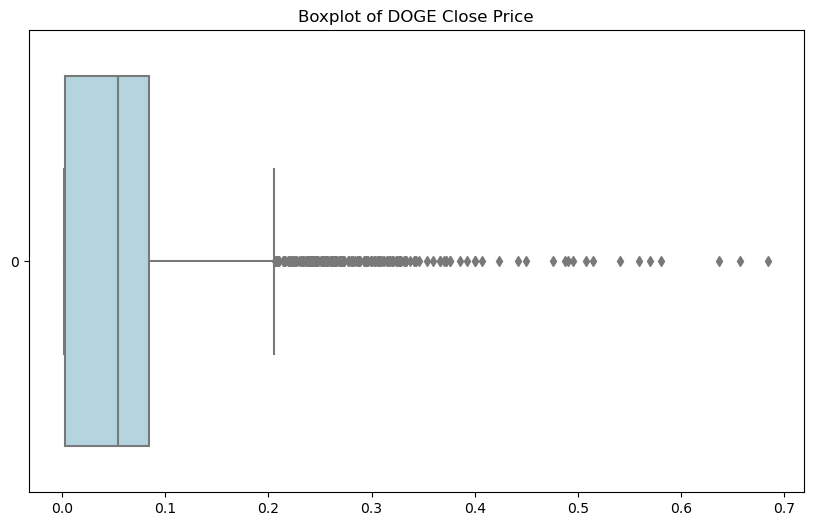
\includegraphics[width=\linewidth]{graph/doge_boxplot.png}
        \caption{DOGE's Box Plot}
        \label{fig:1}
    \end{minipage}
    \hfill
    \begin{minipage}{0.23\textwidth}
        \centering
        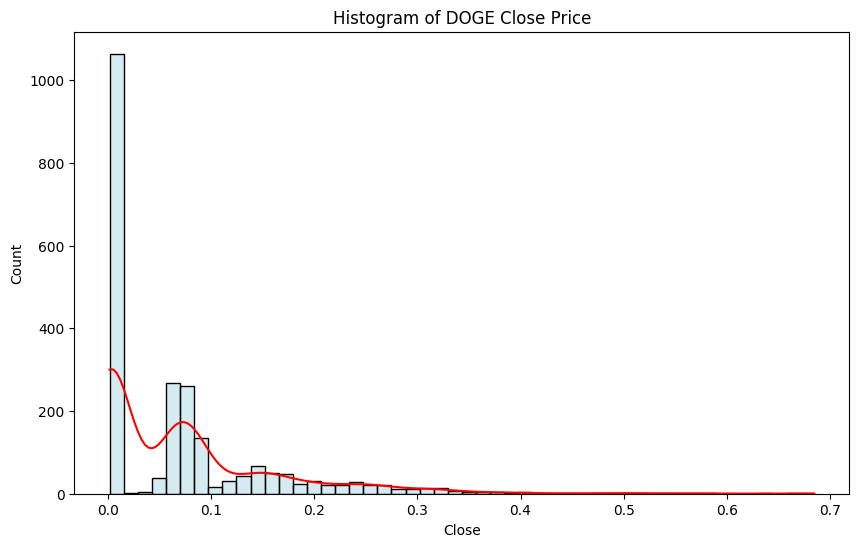
\includegraphics[width=\linewidth]{graph/doge_his.png}
        \caption{DOGE's Histogram}
        \label{fig:2}
    \end{minipage}
\end{figure}

\begin{figure}[H]
    \centering
    \begin{minipage}{0.23\textwidth}
        \centering
        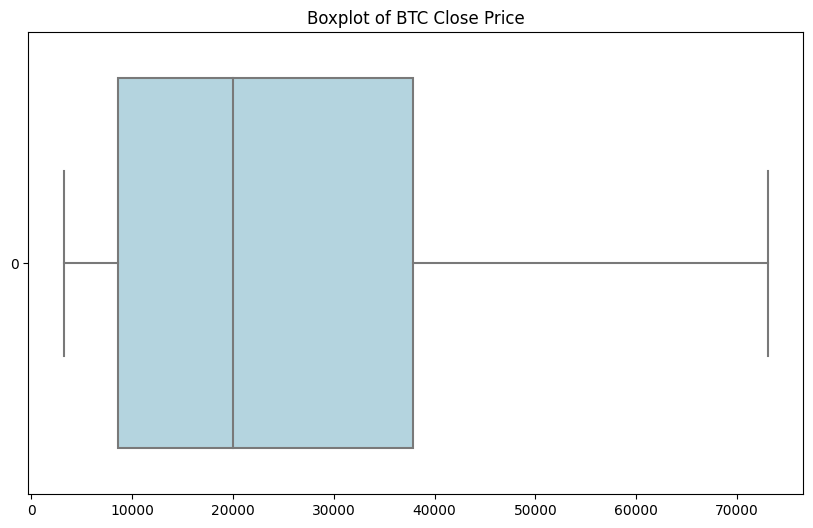
\includegraphics[width=\linewidth]{graph/btc_boxplot.png}
        \caption{BTC's Box Plot}
        \label{fig:3}
    \end{minipage}
    \hfill
    \begin{minipage}{0.23\textwidth}
        \centering
        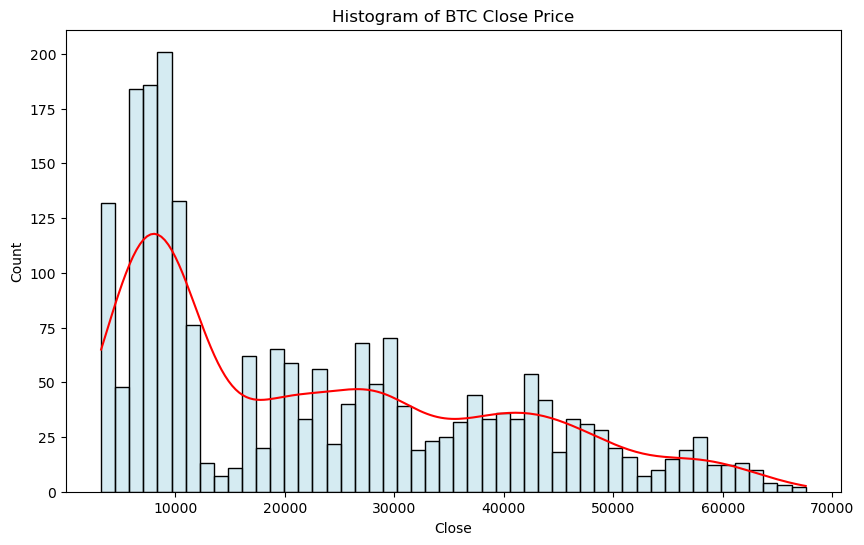
\includegraphics[width=\linewidth]{graph/btc_his.png}
        \caption{BTC's Histogram}
        \label{fig:4}
    \end{minipage}
\end{figure}

\begin{figure}[H]
    \centering
    \begin{minipage}{0.23\textwidth}
        \centering
        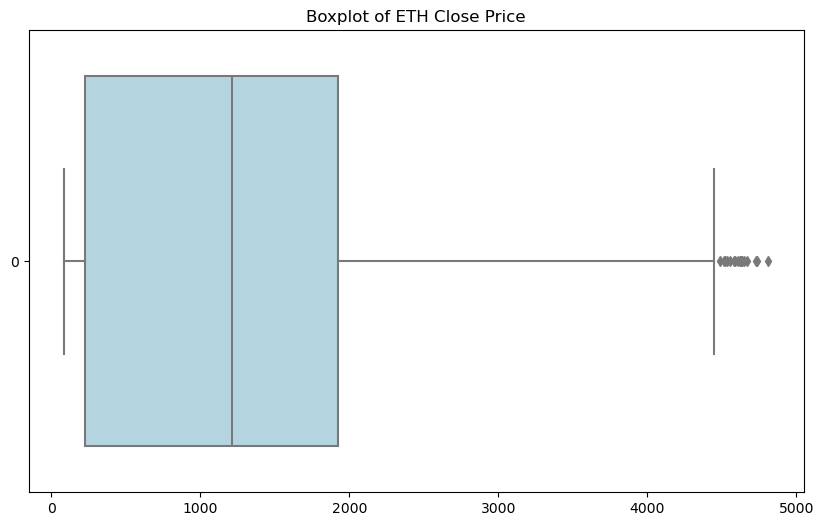
\includegraphics[width=\linewidth]{graph/eth_boxplot.png}
        \caption{ETH's Box Plot}
        \label{fig:5}
    \end{minipage}
    \hfill
    \begin{minipage}{0.23\textwidth}
        \centering
        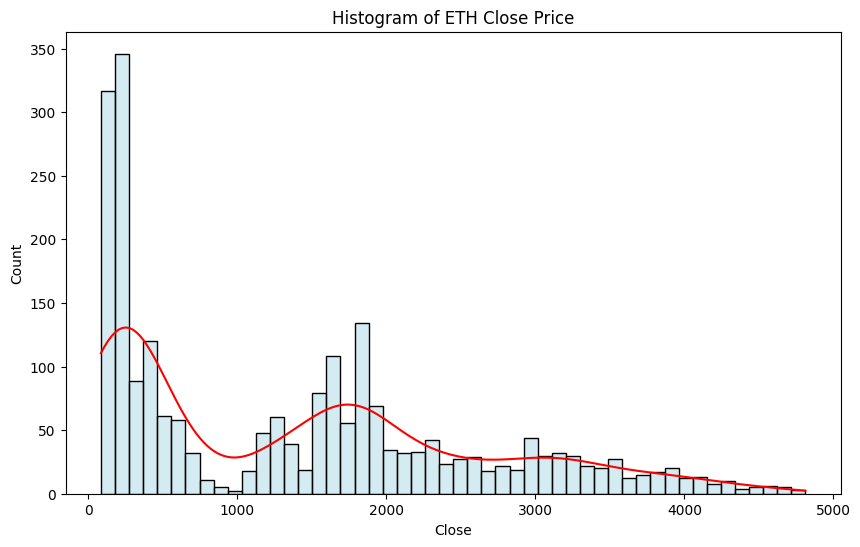
\includegraphics[width=\linewidth]{graph/eth_his.png}
        \caption{ETH's Histogram}
        \label{fig:6}
    \end{minipage}

\end{figure}

\begin{itemize}
    \item Across all three cryptocurrencies, there are remarkable differences in mean values, indicating diverse price levels. Moreover, the considerable range between minimum and maximum values highlights the wide fluctuations in prices, portraying substantial volatility within the market.
    \item The high standard deviation, positive kurtosis, and skewness values suggest non-normal distributions with fat tails and right skewness. This indicates frequent occurrence of outliers and a tendency for prices to be skewed towards higher values, which means the occurrence of high prices isn't significant.
    \item These measures contributes to a summary that it is potential for high profits but also heightened risks when investing in these three cryptocurrencies.

\end{itemize}

\section{Methodology}
\subsection{Linear Regression}
In statistics, Linear Regression is a supervised learning algorithm that simulates a mathematical relationship between a dependent variable and independent
variables, enabling predictions for continuous or numeric variables.\
A multiple linear regression model has the form:
\[Y=\beta_0+\beta_1X_1+\beta_2X_2+\cdots+\beta_kX_k+\varepsilon\]
Where:\\
\indent\textbullet\ Y is the dependent variable (Response variable).\\
\indent\textbullet\ \(X_1, X_2, \ldots, X_k\) are the independent (Explanatory variables).\\
\indent\textbullet\ \(\beta_0\) is the intercept term.\\
\indent\textbullet\ \(\beta_1,..., \beta_k\) are the regression coefficients for the independent variables.\\
\indent\textbullet\ \(\varepsilon\) is the error term.
\subsection{ARIMAX}
\justify
ARIMAX is a time series forecasting model that combines Autoregressive Integrated Moving Average (ARIMA) model with exogenous variables. It extends  ARIMA by  including external  predictors  (denoted as  X) to improve  forecasting accuracy.  This model involves  specifying AR, I,  and MA components,  along with the  exogenous variables, estimating model parameters, and making forecasts \cite{b3}.\\
% ARIMA Models are specified by three order parameters: (p, d, q),\ 

% where,\
%     \indent\textbullet\ p is the order of the AR term
%     \indent\textbullet\ q is the order of the MA term
%     \indent\textbullet\ d is the number of differencing required to make the time series stationary\\

An ARIMAX model depicted by the following equation:
\begin{dmath*}
    Y_t = \alpha
    + \underbrace{\beta_1 X_{1,t} + \ldots + \beta_r X_{r,t}}_{\text{exogenous variables}}
    + \underbrace{\phi_1 Y_{t-1} + \phi_2 Y_{t-2} + \ldots + \phi_p Y_{t-p}}_{\text{AR term}}
    + \underbrace{\varepsilon_t - \theta_1 \varepsilon_{t-1} - \theta_2 \varepsilon_{t-2} - \ldots - \theta_q \varepsilon_{t-q}}_{\text{MA term}}
\end{dmath*}

\subsection{Vector Autoregression}
Vector Autoregression (VAR) is a multivariate forecasting algorithm that is used when two or more time series influence each other. \\
It is considered as a generalization of univariate AR models or a combination between the two or more models and the univariate time series models. Each variable in a VAR is explained by its own lagged values and the lagged values of all the other variables in the equation.\cite{b8} The basic VAR (p) model is given by:
\[Y_t=c+A_1y_{t-1}+A_2y_{t-2}+...+A_py_{t-p}+\varepsilon_t\]
Where:\\
\indent\textbullet\ \(y_t-i\): the "ith lag" of \(y_t\)\\
\indent\textbullet\ \(c\) is a k-vector of constants\\
\indent\textbullet\ \(A_i\): time-invariant (k × k)-matrix\\
\indent\textbullet\ \(\boldsymbol{\varepsilon}_t\): a vector of error terms with \(k\) element\\
In matrix form:\\
\begin{dmath*}
    Y_t=\left[\begin{matrix}y_1\\y_2\\\begin{matrix}\begin{matrix}.\\.\\\end{matrix}\\y_k\\\end{matrix}\\\end{matrix}\right]\ =\left[\begin{matrix}c_1\\c_2\\\begin{matrix}\begin{matrix}.\\.\\\end{matrix}\\c_k\\\end{matrix}\\\end{matrix}\right]+\left[\begin{matrix}\begin{matrix}\phi_{11}\\\phi_{21}\\\end{matrix}&\begin{matrix}.\\.\\\end{matrix}&\begin{matrix}.\\.\\\end{matrix}\\\begin{matrix}.\\.\\\end{matrix}&\ &\ \\\phi_{k1}&.&.\\\end{matrix}\right]\left[\begin{matrix}y_{1,t-1}\\y_{2,t-1}\\\begin{matrix}\begin{matrix}.\\.\\\end{matrix}\\y_{k,t-1}\\\end{matrix}\\\end{matrix}\right]+...+\ \left[\begin{matrix}\begin{matrix}\phi_{11}\\\phi_{21}\\\end{matrix}&\begin{matrix}.\\.\\\end{matrix}&\begin{matrix}.\\.\\\end{matrix}\\\begin{matrix}.\\.\\\end{matrix}&\ &\ \\\phi_{k1}&.&.\\\end{matrix}\right]\left[\begin{matrix}y_{1,t-p}\\y_{2,t-p}\\\begin{matrix}\begin{matrix}.\\.\\\end{matrix}\\y_{k,t-p}\\\end{matrix}\\\end{matrix}\right]+\left[\begin{matrix}\varepsilon_1\\\varepsilon_2\\\begin{matrix}\begin{matrix}.\\.\\\end{matrix}\\\varepsilon_k\\\end{matrix}\\\end{matrix}\right]
\end{dmath*}

\subsection{Recurrent Neural Networks (RNN)}
Recurrent Neural Networks (RNNs) are a class of artificial neural networks designed for sequential data, where the connections between nodes form a directed graph along a temporal sequence. This allows RNNs to exhibit temporal dynamic behavior for a time sequence.\ 
\begin{figure}[h]
    \centering
    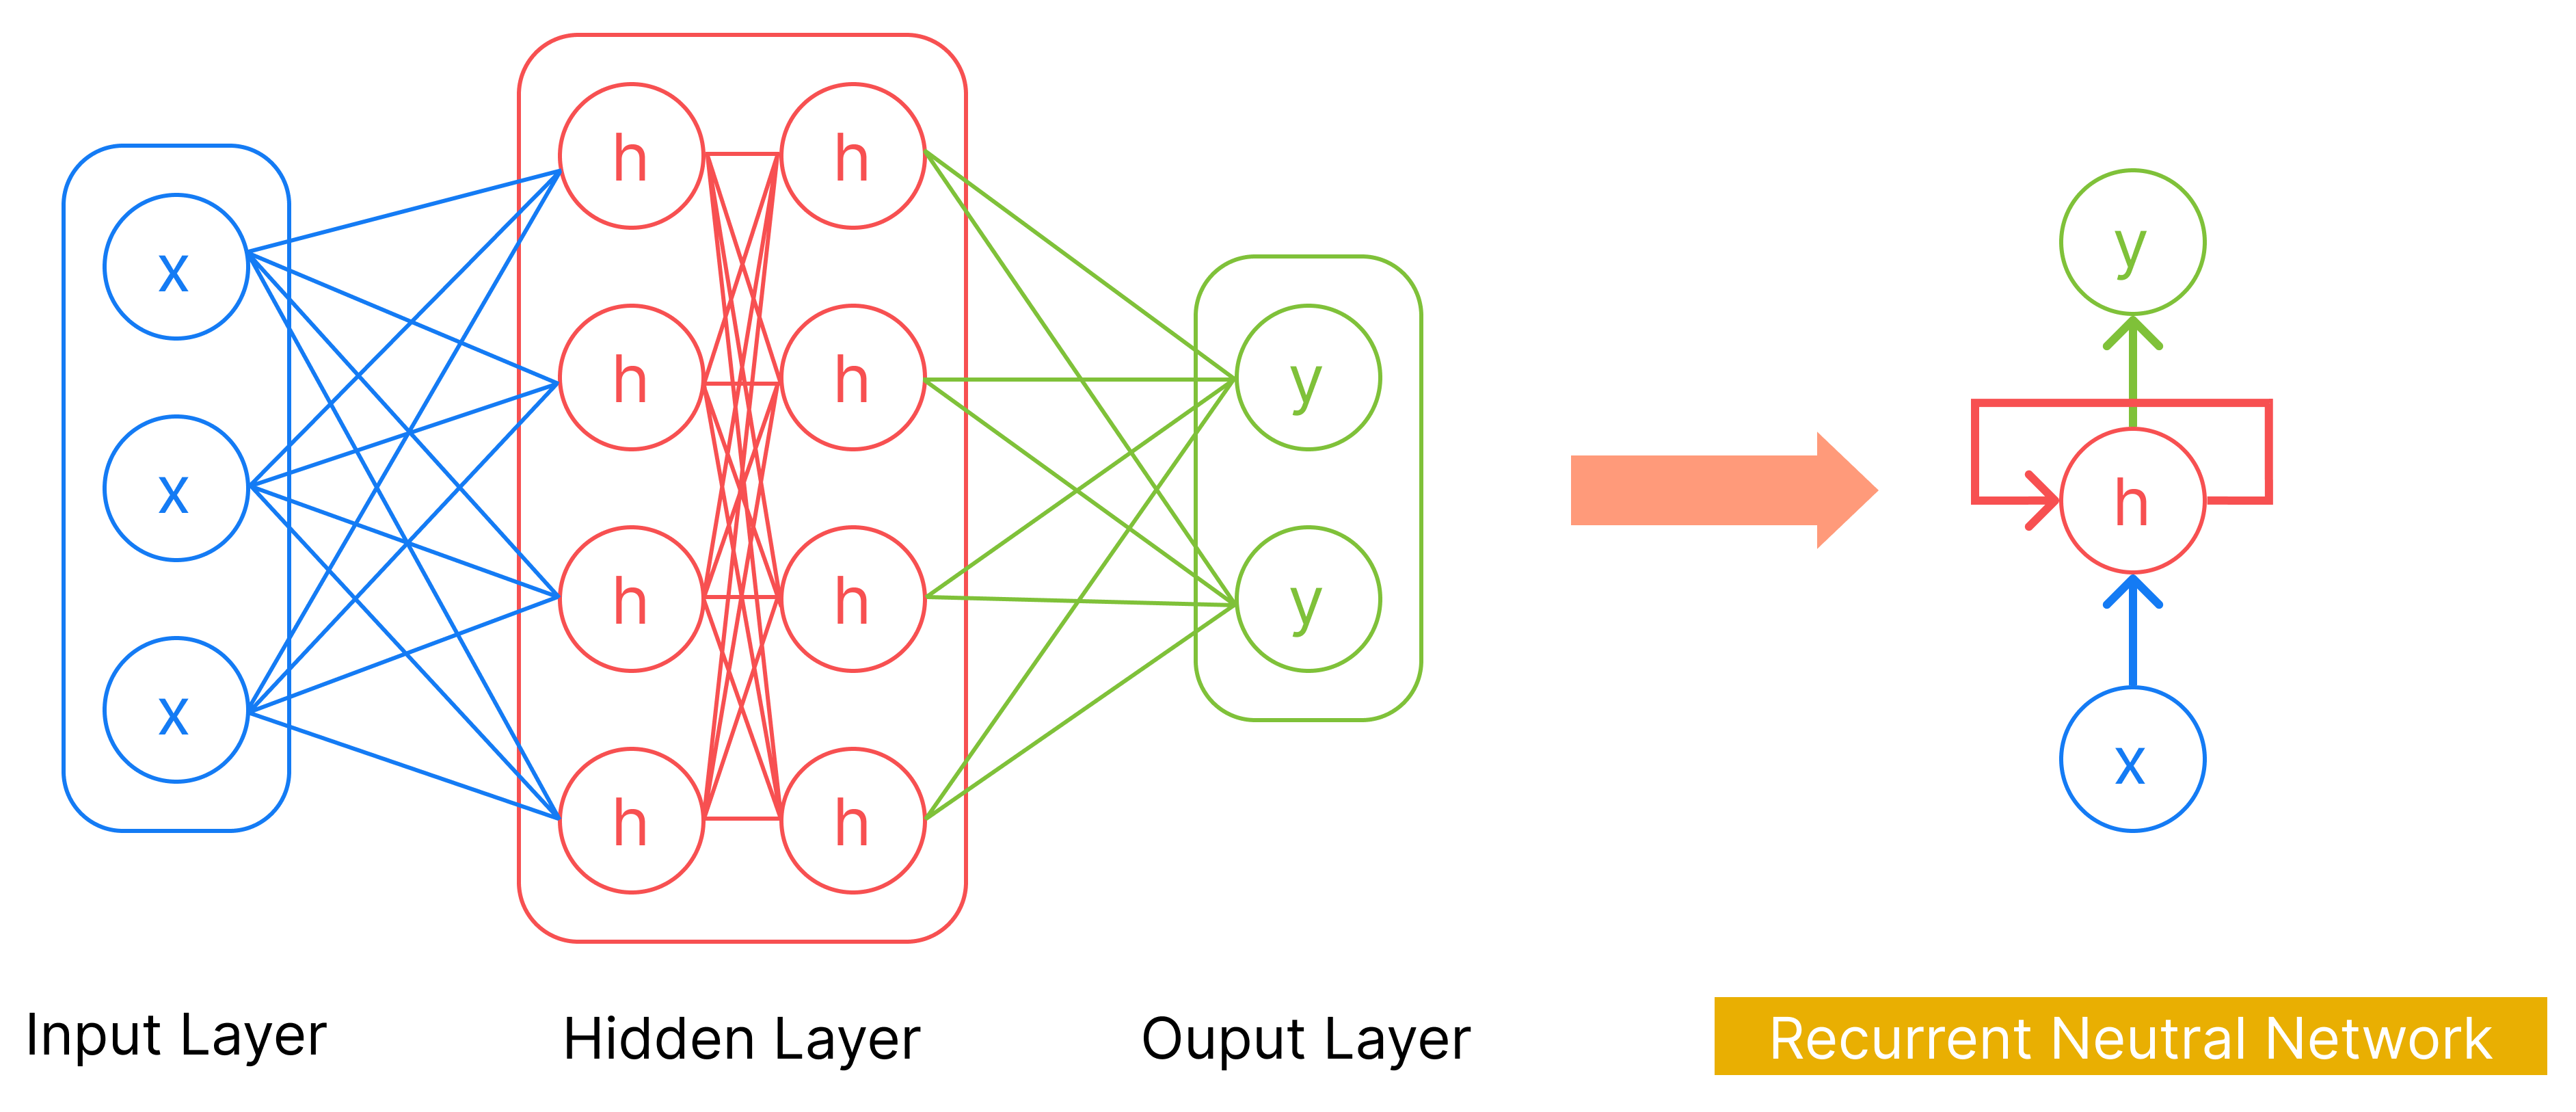
\includegraphics[width=\linewidth]{./image/RNN.png}
    \caption{Model of RNN architectural}
    \label{fig:7}
\end{figure}\\
\begin {itemize}
    \item \textbf{Input Layer}: Networks have only one input layer.
    \item \textbf{Hidden Layer}: Networks have multiple hidden layers.
    \item \textbf{Output Layer}: Networks have only one output layer.
\end {itemize}
A basic RNN can be represented as follows:
\begin{dmath*}
    h_t = f(W_{xh} x_t + W_{hh} h_{t-1} + b_h)
\end{dmath*}
\begin{dmath*}
    y_t = g(W_{hy} h_t + b_y)
\end{dmath*}
Where:\begin {itemize}
\item \(x_t\) is the input at time step \(t\).
\item \(h_t\) is the hidden state at time step \(t\).
\item \(y_t\) is the output at time step \(t\).
\item \(W_{xh}\), \(W_{hh}\), and \(W_{hy}\) are weight matrices.
\item \(b_h\) and \(b_y\) are bias vectors.
\item \(f\) and \(g\) are activation functions.
\end{itemize}

\subsection{Long Short-Term Memory (LSTM)}
Long Short-Term Memory (LSTM) networks are a type of RNN designed to address the vanishing gradient problem that can occur with traditional RNNs when processing long sequences. LSTMs achieve this through a memory cell which is controlled by three gates:\\
\begin{figure}[H]
    \centering
    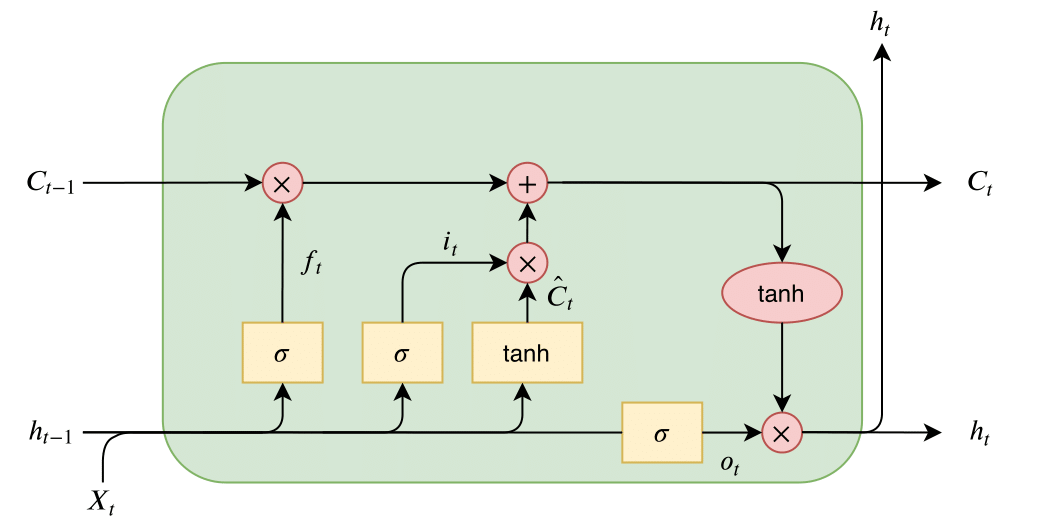
\includegraphics[width=0.8\linewidth]{./image/LSTM.png}
    \caption{Model of LSTM architectural}
    \label{fig:8}
\end{figure}
\noindent
- \textbf{Forget Gate}: Controls what information is discarded from the cell state.
\begin{dmath*}
    f_t = \sigma(W_f \cdot [h_{t-1}, x_t] + b_f)
\end{dmath*}
- \textbf{Input Gate}: Controls what new information is added to the cell state.
\begin{dmath*}
    i_t = \sigma(W_i \cdot [h_{t-1}, x_t] + b_i)
\end{dmath*}
\begin{dmath*}
    \tilde{C}_t = \tanh(W_C \cdot [h_{t-1}, x_t] + b_C)
\end{dmath*}
- \textbf{Output Gate}: Controls what information is output form the cell state.
\begin{dmath*}
    o_t = \sigma(W_o \cdot [h_{t-1}, x_t] + b_o)
\end{dmath*}
Where:
\begin{itemize}
    \item \(W_f\), \(W_i\), \(W_C\), \(W_o\) are the weight matrices of \textbf{f}orget gate, \textbf{i}nput gate, \textbf{C}ell state, and \textbf{o}utput gate respectively.
    \item \(b_f\), \(b_i\), \(b_C\), \(b_o\) are the bias vectors of  \textbf{f}orget gate, \textbf{i}nput gate, \textbf{C}ell state, and \textbf{o}utput gate respectively.
    \item \(\sigma\) is the sigmoid activation function.
    \item \(\tanh\) is tanh activation function that gives an output of vector from -1 to +1.
\end{itemize}
Then the cell state \(C_t\) and hidden state \(h_t\) are then updated as follows:
\begin{dmath*}
    C_t = f_t * C_{t-1} + i_t * \tilde{C}_t
\end{dmath*}
\begin{dmath*}
    h_t = o_t * \tanh(C_t)
\end{dmath*}

\subsection{Gated Recurrent Unit (GRU)}
Gated Recurrent Units (GRUs) are another type of RNN with a simplified gating mechanism compared to LSTMs, which selectively update the hidden state at each time step. The GRU has only two gating mechanisms:\\
\begin{figure}[H]
    \centering
    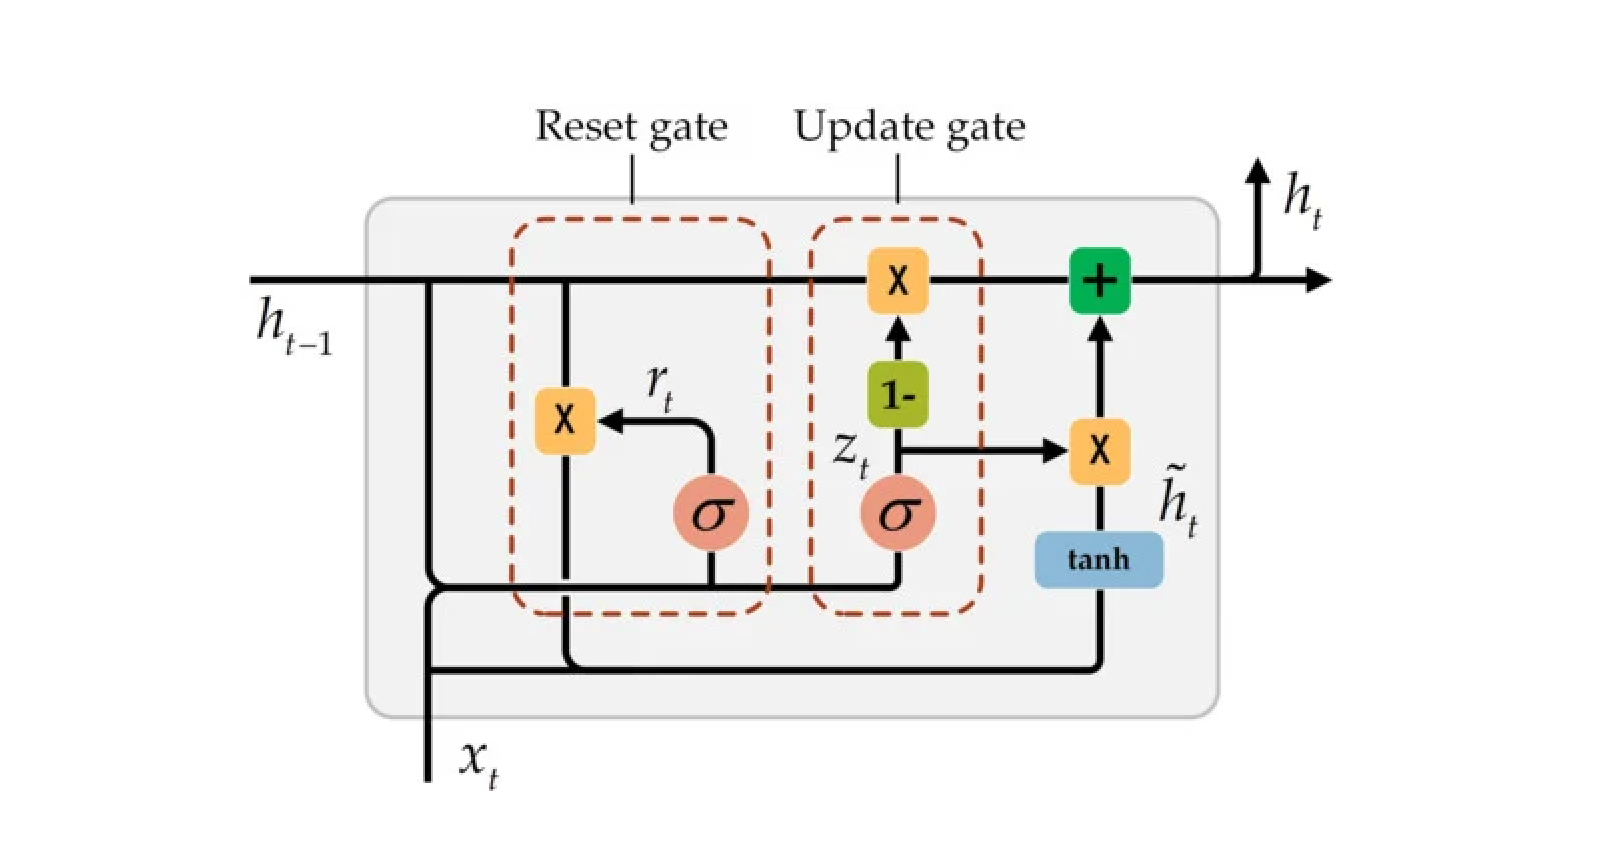
\includegraphics[width=\linewidth]{./image/GRU.png}
    \caption{Model of GRU architectural}
    \label{fig:9}
\end{figure}
\noindent
- \textbf{Update Gate}: Controls the amount of information from the previous hidden state to let through, and the amount of new information to add.
\begin{dmath*}
    z_t = \sigma(W_z \cdot [h_{t-1}, x_t] + b_z)
\end{dmath*}
- \textbf{Reset Gate}: Controls the amount of information to forget from the previous hidden state.
\begin{dmath*}
    r_t = \sigma(W_r \cdot [h_{t-1}, x_t] + b_r)
\end{dmath*}
The candidate hidden state is calculated based on the reset gate and the previous hidden state.
\begin{dmath*}
    \tilde{h}_t = \tanh(W \cdot [r_t * h_{t-1}, x_t] + b)
\end{dmath*}
Then the hidden state is updated based on the update gate and the candidate hidden state.
\begin{dmath*}
    h_t = (1 - z_t) * h_{t-1} + z_t * \tilde{h}_t
\end{dmath*}
Where:
\begin{itemize}
    \item \(z_t\) and \(r_t\) are the update gate and reset gate.
    \item \(W_z\), \(W_r\), \(W\), \(b_z\), \(b_r\), \(b\) are the weight matrices and bias vectors of the update gate, reset gate, and candidate hidden state respectively.
    \item \(\sigma\) is the sigmoid activation function.
    \item \(\tanh\) is the hyperbolic tangent activation function.
\end{itemize}
\subsection{XGBoost}
XGBoost (eXtreme Gradient Boosting) is a powerful machine learning algorithm that uses an ensemble of decision trees and gradient boosting, which combines multiple weak learners to create a strong predictive model, to minimize prediction errors \cite{b9}.\\
\begin{figure} [H]
    \centering
    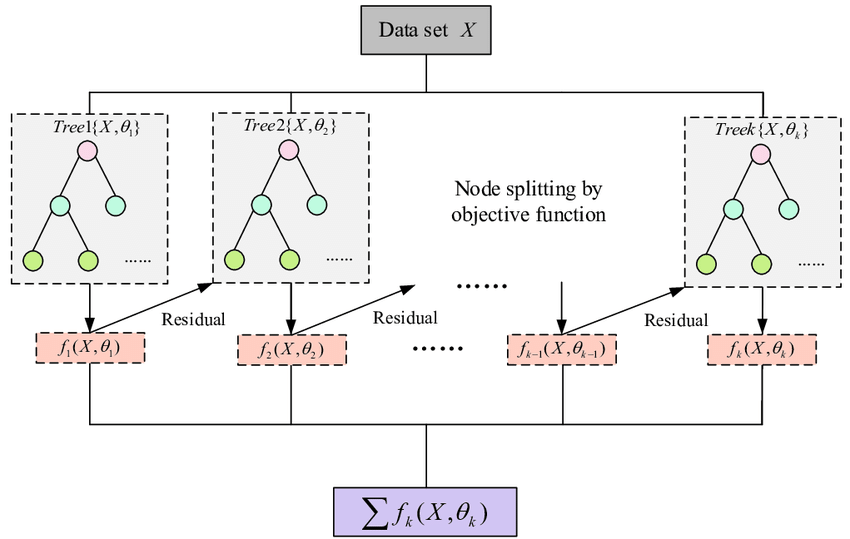
\includegraphics[width=0.8\linewidth]{./image/XGBoost.png}
    \caption{Model of XGBoost architectural}
    \label{fig:10}
\end{figure}
\noindent
- \textbf{Loss Function}: Measures the difference between the true label \(y_i\) and the predicted label \(\hat{y}_i\),\\
\begin{dmath*}
    l(y_i, \hat{y}_i) 
\end{dmath*}
- \textbf{Regularization Term}: Penalizes model complexity to prevent overfitting in each the \(f\) tree.\\
\begin{dmath*}
    \Omega(f) = \gamma T + \frac{1}{2} \lambda ||w||^2
\end{dmath*}
Where:
\begin{itemize}
    \item \(T\) is the number of leaves in the \(f\) tree.
    \item \(w\) is the leaf weight of the \(f\) tree.
    \item \(\lambda\), \(\gamma\)  are the  hyperparameters.
\end{itemize}
- \textbf{Objective Function} = Loss Function + Regularization Term
\begin{dmath*}
    \mathcal{L}(\phi) = \sum_{i=1}^n l(y_i, \hat{y}_i) + \Omega(f_k)
\end{dmath*}
Decision trees are built sequentially to minimize the objective function. At each step, a new tree \(f_t\) with input features \(x_i\) is added to correct the errors of the current model.
\begin{dmath*}
    \hat{y}_i^{(t)} = \hat{y}_i^{(t-1)} + f_t(x_i)
\end{dmath*}
- \textbf{Second-order Taylor expansion} is used to optimized the objective function based on gradient \(g\) and hessian \(h\) of the loss function.
\begin{dmath*}
    \mathcal{L}^{(t)} \approx \sum_{i=1}^n [l(y_i, \hat{y}_i^{(t-1)}) + g_i f_t(x_i) + \frac{1}{2} h_i f_t^2(x_i)] + \Omega(f_t)
\end{dmath*}
Where:
\begin{itemize}
    \item \(n\) is the number of data instances.
    \item \(g_i\) = \(\frac{\partial l(y_i, \hat{y}_i)}{\partial \hat{y}_i}\) and \(h_i\) = \(\frac{\partial^2 l(y_i, \hat{y}_i)}{\partial \hat{y}_i^2}\)
\end{itemize}
And to find the optimal leaf weight \(w_j\) for each leaf node \(j\), the objective function is minimized. Then we have the equation:
\begin{dmath*}
    w_j = -\frac{\sum_{i \in I_j} g_i}{\sum_{i \in I_j} h_i + \lambda}
\end{dmath*}
\subsection{LightGBM}
LightGBM (Light Gradient Boosting Machine) is a gradient-boosting framework, based on decision tree algorithms, that uses a histogram-based algorithm to speed up training and reduce memory usage. It splits the tree leaf-wise, rather than level-wise, to minimize loss and improve accuracy.\\
\begin{figure}[H]
    \centering
    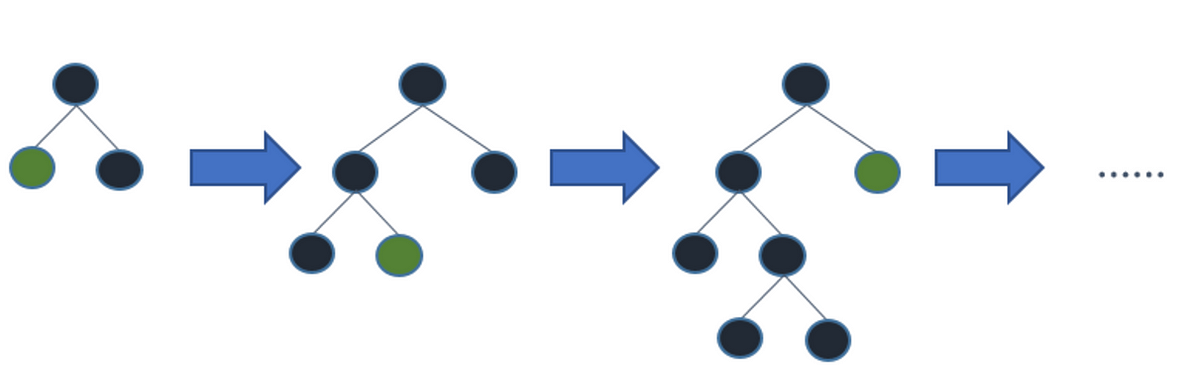
\includegraphics[width=0.8\linewidth]{./image/LightGBM.png}
    \caption{Leaf-wise tree expansion in LightGBM}
    \label{fig:11}
\end{figure}
\noindent
Additionally, LightGBM combines two techniques to improve performance of GBDT: Gradient-based One-Side Sampling (GOSS) and Exclusive Feature Bundling (EFB).\\
- \textbf{GOSS}: Retains all instances with large gradients and samples a subset of instances with small gradients to reduce the number of instances.\\
- \textbf{EFB}: Bundles exclusive features to reduce the number of features and improve efficiency.
\section{Experiment}
\subsection{Feature Engineering}
\subsection {Dataset Split Ratio}
\subsection {Evaluation Methods}
\subsection {Results}

\section{Conclusion}

\subsection{Summary}

\subsection{Future Considerations}

\section*{Acknowledgment}


%% UNCOMMENT these lines below (and remove the 2 commands above) if you want to embed the bibliografy.
\begin{thebibliography}{00}
    \bibitem{b1} Sun, G. (2024). Cryptocurrency price prediction based on Xgboost, LightGBM and BNN. \textit{Applied and Computational Engineering}, 49(1), 273–279. \url{https://doi.org/10.54254/2755-2721/49/20241414}

    \bibitem{b2} Yuan, Z. (2023). Gold and Bitcoin Price Prediction based on KNN, XGBoost and LightGBM Model. \textit{Highlights in Science, Engineering and Technology}, 39, 720–725. \url{https://doi.org/10.54097/hset.v39i.6635}

    \bibitem{b3} Haydier, E., Albarwari, N., \& Ali, T. H. (2023, December 1). The Comparison Between VAR and ARIMAX Time Series Models in Forecasting. \textit{Iraqi Journal of Statistical Sciences}. \url{https://doi.org/10.33899/iqjoss.2023.181260}

    \bibitem{b4} Dutta, A., Kumar, S. S., \& Basu, M. (2020). A gated Recurrent unit approach to bitcoin price prediction. \textit{Journal of Risk and Financial Management}, 13(2), 23. \url{https://doi.org/10.3390/jrfm13020023}

    \bibitem{b5} Gunarto, D. M., Saadah, S., \& Utama, D. Q. (2023). Predicting cryptocurrency price using RNN and LSTM method. \textit{Jurnal Sistem Informasi Dan Komputer/Jurnal Sisfokom}, 12(1), 1–8. \url{https://doi.org/10.32736/sisfokom.v12i1.1554}

    \bibitem{b6} Huang, J.-Z., Huang, W., \& Ni, J. (2019). Predicting bitcoin returns using high-dimensional technical indicators. \textit{The Journal of Finance and Data Science}, 5(3), 140–155. \url{https://doi.org/10.1016/j.jfds.2018.10.001}

    \bibitem{b7} Mudassir, M., Bennbaia, S., Ünal, D., \& Hammoudeh, M. (2020). Time-series forecasting of Bitcoin prices using high-dimensional features: a machine learning approach. \textit{Neural Computing and Applications}. \url{https://doi.org/10.1007/s00521-020-05129-6}

    \bibitem{b8} Metsileng, L. D., Moroke, N. D., \& Tsoku, J. T. (2018). Modelling the BRICS exchange rates using the Vector Autoregressive (VAR) model. \textit{Journal of Economics and Behavioral Studies}, 10(5(J)), 220–229. \url{https://doi.org/10.22610/jebs.v10i5(j).2511}

    \bibitem {b9} What is XGBoost? (n.d.). NVIDIA Data Science Glossary. \url{https://www.nvidia.com/en-us/glossary/xgboost/}

    \bibitem{b10} Chen, T., \& Guestrin, C. (2016, August). Xgboost: A scalable tree boosting system. \textit{In Proceedings of the 22nd acm sigkdd international conference on knowledge discovery and data mining (pp. 785-794).} 

\end{thebibliography}

\EOD

\end{document}
